\section{Feature-Sensitive Coverage Criteria}\label{sec:fscov}

This section formulates a general definition of graph coverage
for a directed graph and explains representative coverage criteria as examples.
Then, we introduce \textit{feature-sensitive (FS) coverage} criteria as general
extensions of graph coverage criteria to discriminate semantics between
different language features.
Finally, we define \textit{feature-call-path-sensitive (FCPS) coverage}
criteria as variants of FS coverage criteria to distinguish different parts in
the semantics of the same language feature.


%----------------------------------------%
%----------------------------------------%


\subsection{Notations}\label{sec:notation}
%
First, we define notations used in the definition of graph coverage criteria.
%
A \textit{directed graph} $\graph = (\nodeset, \inodeset,
\fnodeset, \edgeset)$ consists of:
\begin{itemize}
  \item a set of \textit{nodes} $\nodeset$
  \item a set of \textit{initial nodes} $\inodeset \subseteq \nodeset$
  \item a set of \textit{final nodes} $\fnodeset \subseteq \nodeset$
  \item a set of \textit{edges} $\edgeset \subseteq \nodeset \times \nodeset
    \times (\annotset \uplus \{ \bot \})$ with a set of \textit{annotations}
    $\annotset$
\end{itemize}
%
The notation $\node \edge{\annot} \node'$ denotes an edge from a node $\node$ to
a node $\node'$ with an annotation $\annot \in \annotset$.
%
If an edge has an empty annotation $\bot$, we omit the annotation: $\node
\edge{} \node'$.
%
In a given directed graph $\graph$, a \textit{path} $\pat \in \patset{\graph}$
is a sequence of one or more nodes, where each pair of adjacent nodes is an
edge:
\begin{equation}\label{euq:path-def}
  \patset{\graph} = \{
    \node_0 \edge{\annot_0} \cdots \edge{\annot_{m-1}} \node_m \mid
    \forall i < m. \; \node_i \edge{\annot_i} \node_{i+1} \in \edgeset \wedge
    \node_m \in \nodeset
  \}
\end{equation}
%
The length of a path is defined as $\norm{\node_0 \edge{\annot_0} \cdots
\edge{\annot_{m-1}} \node_m} = m$.
%
A path $\pat$ is a \textit{subpath} ($\subpath$) of a path $\pat'$ when $\pat$
is a subsequence of $\pat'$.
%
We use the notation $\prefix$ for a prefix relation, and $\getfirst(\pat)$ and
$\getlast(\pat)$ denote the first and last nodes of the path $\pat$,
respectively.
%
A path $\pat$ is \textit{full} when it starts at an initial node and ends at a
final node: $\getfirst(\pat) \in \inodeset \wedge \getlast(\pat) \in \fnodeset$.
%
Then, $\patmap{\graph} : \testset \rightarrow \patset{\graph}$ is a mapping from
a \textit{test} $\test \in \testset$ to a full path in the graph $\graph$, and
we call $\patmap{\graph}(\test)$ the \textit{execution path} of $\test$.

%----------------------------------------%

\paragraph{\textbf{Example}}
%
Consider the CFG $\graph$ in Figure~\ref{fig:spec-cfg}
and the following JavaScript programs as a test set $T
\subseteq \testset$:
\begin{equation}\label{equ:testset}
  T = \{
    \cdots,
    \underset{\addtest}{\underline{\jscode{2n + 1}}},
    \underset{\subtest}{\underline{\jscode{2n - 1}}},
    \cdots
  \}
\end{equation}
%
Then, $\patmap{\graph}(\addtest)$, the execution path of $\addtest$, is
depeicted as follows:
\[
  \small
  \!\begin{array}{l}
    \cdots
    \call \overset{\text{{\bf Evaluation} of \esnt{AdditiveExpression}
      \esconst{+} \esnt{MultiplicativeExpression}}}{\rcolorbox{gray3}{\(
    1
    \call
    \overset{\textbf{EvaluateStringOrNumericBinaryExpression}}{\rcolorbox{gray2}{\(
    7 \edge{} \cdots \edge{} 8
    \call \overset{\textbf{ApplyStringOrNumericBinaryOperator}}{\colorbox{gray1}{\(
    11 \edge{} \cdots \edge{} 12
    \call \overset{\textbf{ToNumeric}}{\colorbox{white}{\(
    19 \edge{} \cdots \edge{} 20 \tedge \colorbox{lightred}{21} \edge{} 22
    \)}}
    \ret 13 \fedge 14
    \)}}
    \)}}
    \)}}

    \vspace*{1em}\\

    \lcolorbox{gray3}{\(
    \lcolorbox{gray2}{\(
    \colorbox{gray1}{\(
    \call \overset{\textbf{ToNumeric}}{\colorbox{white}{\(
    19 \edge{} \cdots \edge{} 20 \fedge \cdots \edge{} 22
    \)}}
    \ret 15 \fedge 16 \tedge \colorbox{lightred}{17} \edge{} 18
    \)}
    \ret 9 \tedge 10
    \)}
    \ret 2 \tedge 3
    \)}
    \ret \cdots\\
  \end{array}
\]
And, $\patmap{\graph}(\subtest)$ is equal to $\patmap{\graph}(\addtest)$ except
for nodes labeled 4, 5, and 6 in the $\textbf{Evaluation}$ SDO for subtraction
rather than 1, 2, and 3 in the $\textbf{Evaluation}$ SDO for addition.
%
The following path $\pat$ is a subpath of both $\patmap{\graph}(\addtest)$ and
$\patmap{\graph}(\subtest)$:
\begin{equation}\label{equ:subpath}
  \pat = 22 \ret 15 \fedge 16 \tedge \colorbox{lightred}{17}
\end{equation}
whose length is $\norm{\pat} = 3$.


%----------------------------------------%
%----------------------------------------%


\subsection{Graph Coverage Criteria}\label{sec:cov}

We formulate graph coverage criteria by referring to their well-known
definitions~\cite{cov-def}.
%
For a given directed graph, we specify a \textit{graph coverage} criterion by 1)
a set of \textit{test requirements} and 2) a \textit{cover relation} between
paths and test requirements:

%----------------------------------------%

\begin{definition}[Graph Coverage Criteria]\label{def:graph-cov}
  A \textit{graph coverage} criterion $\cov{\graph} = (\trset{\graph}, \cover)$
  for a given directed graph $\graph$ is defined with:
  \begin{itemize}
    \item a set of \textit{test requirements (TRs)} $\trset{\graph}$
    \item a \textit{cover relation} $\cover \subseteq \patset{\graph} \times
      \trset{\graph}$ between paths and TRs
  \end{itemize}
\end{definition}

%----------------------------------------%

In a specific graph coverage criterion $\cov{\graph}$, we say that a path $\pat$
\textit{covers} a TR $\tr \in \trset{\graph}$ when $\pat \cover
\tr$.
A test $\test \in \testset$ covers the TR $\tr$ if there exists
a prefix path $\pat$ of its execution path that covers the TR:
%
\begin{equation}\label{equ:test-cover}
  \test \cover \tr
  \iff
  \exists \pat \in \patset{\graph}. \tst
  \pat \prefix \patmap{\graph}(\test) \wedge
  \pat \cover \tr
\end{equation}
%
A test set $T \subseteq \testset$ \textit{satisfies} ($\sat$) the criterion
$\cov{\graph}$ when it covers all valid TRs:
\begin{equation}\label{equ:sat}
  T \sat \cov{\graph}
  \iff
  \forall \tr \in \trset{\graph}. \;
  \tr \; \text{is valid} \; \Rightarrow
  \exists \test \in T. \tst \test \cover \tr
\end{equation}
where a TR $\tr$ is \textit{valid} if there exists a possible test $\test \in
\testset$ that covers $\tr$.
%
If $T \sat \cov{\graph} \Rightarrow T \sat \cov{\graph}'$ for any test set $T$,
we say that $\cov{\graph}$ \textit{subsumes} $\cov{\graph}'$ and use the
notation: $\cov{\graph} \subs \cov{\graph}'$.
%
The subsumption relation between graph coverage criteria is a partial order.

%----------------------------------------%

\begin{definition}[Node Coverage]\label{def:node-cov} In a \textit{node
  coverage} criterion $\nodecov{\graph}$,
  \begin{itemize}
    \item the set of \textbf{TRs} $\trset{\graph}$ is a set of nodes:
      $  \trset{\graph} = \nodeset $
    \item a path $\pat$ \textbf{covers} a node $\node$ when it ends with the
      node $\node$:
      $  \pat \cover \node \iff \getlast(\pat) = \node $
  \end{itemize}
\end{definition}

%----------------------------------------%

The \textit{node coverage} criterion is the most common graph coverage criterion
whose test requirements are nodes, and we can generalize it into
\textit{$k$-limiting path coverage} criteria using paths:

%----------------------------------------%

\begin{definition}[$k$-Limiting Path Coverage]\label{def:k-path-cov}
  In a \textit{$k$-limiting path coverage} criterion $\kpathcov{k}{\graph}$,
  \begin{itemize}
    \item the set of \textbf{TRs} $\trset{\graph}$ is a set of
      paths whose lengths are bounded by $k$:
$
        \trset{\graph} = \{ \pat \in \patset{\graph} \mid \norm{\pat} \leq k \}
$
    \item a path $\pat$ \textbf{covers} a path $\pat'$ when their last nodes are
      equal and the path $\pat'$ is a subpath of $\pat$:
$
        \pat \cover \pat'
        \iff
        \getlast(\pat) = \getlast(\pat') \wedge \pat' \subpath \pat
$
  \end{itemize}
\end{definition}

%----------------------------------------%

Now, the node coverage criterion can be redefined as the 0-limiting path
coverage criterion ($\kpathcov{0}{\graph} = \nodecov{\graph}$), and other graph
coverage criteria match with $k$-limiting path coverages as well:
\begin{itemize}
  \item The \textit{edge coverage} criterion is $\kpathcov{1}{\graph}$
  \item The \textit{edge-pair coverage} criterion is $\kpathcov{2}{\graph}$
  \item The \textit{complete path coverage} criterion is
    $\kpathcov{\infty}{\graph}$
\end{itemize}
%
Note that $k$-limiting path coverage criteria utilize the inequality for path
lengths $\norm{\pat} \leq k$ rather than equality $\norm{\pat} = k$.
%
Thus, if $i \leq j$, the set of TRs in $\kpathcov{i}{\graph}$ is always a subset
of that in $\kpathcov{j}{\graph}$, and $\kpathcov{j}{\graph}$ subsumes
$\kpathcov{i}{\graph}$.
%
The \textit{branch coverage} criterion is a variant of the edge coverage
criterion that treats only out-edges of conditional branches as TRs.
%
It is possible to merge multiple coverage criteria by defining unions of their
TRs and cover relations.
%
For example, a \textit{node-or-branch coverage} criterion is a merge
of node and branch coverage criteria.

%----------------------------------------%

The complete path coverage criterion might have infinite TRs because of
recursions and loop structures.
%
To resolve this problem, \citet{cov-def} have presented a \textit{simple path
coverage} criterion that considers only simple paths as TRs.
%
A path $\node_0 \edge{\annot_0} \cdots \edge{\annot_{m-1}} \node_m$ is
\textit{simple} if there are no duplicated nodes in the path, with the exception that the
first and last nodes may be identical: $\forall i, j. \; \node_i = \node_j
\Rightarrow (i = j \vee \{ i, j \} = \{ 0, m \})$.
%
In addition, they extend it to a \textit{prime path coverage} criterion to
reduce the number of TRs by filtering out duplicated simple paths, where a
\textit{prime path} is a maximal length simple path in the graph.
%
However, even such advanced structural coverage criteria still need many
TRs for the entire control-flow graphs.
%
Hence, they are usually used for unit testing~\cite{unit-test} in practice
with intra-procedural control-flow graphs.

%----------------------------------------%

\paragraph{\textbf{Example}}
%
Consider the CFG $\graph$ in Figure~\ref{fig:spec-cfg} and the test
set $T$ in (\ref{equ:testset}), including $\addtest$ and $\subtest$.
%
If we measure the 3-limiting path coverage $\kpathcov{3}{\graph}$ for
$T$, both the node labeled 17 and the path $\pat$ in (\ref{equ:subpath}) are
test requirements $\trset{\graph}$.
%
First, the prefix path, whose last node is 17, of $\patmap{\graph}(\addtest)$
covers both TRs: the node labeled 17 and $\pat$.
%
Thus, the test $\addtest$ for addition covers both of them.
%
Similarly, the test $\subtest$ for subtraction covers both of them for the same
reason.
%
Unfortunately, either $\addtest$ or $\subtest$ might be removed in the program
pool because they cover the same TRs, the node labeled 17 and the path $\pat$.


%----------------------------------------%
%----------------------------------------%


\subsection{Feature-Sensitive (FS) Coverage Criteria}\label{sec:fs-cov}

To alleviate the problem introduced in Section~\ref{sec:diff-feat}, we present
\textit{feature-sensitive (FS) coverage} criteria as general extensions of any
graph coverages depending on the following three components:
%
\begin{itemize}
  \item a given graph coverage criterion $\cov{\graph}$
  \item a set of \textit{language features} $\featset$
  \item a \textit{feature mapping} $\featmap: \nodeset \rightarrow \featset
    \uplus \{ \bot \}$, a partial mapping from nodes to language features
\end{itemize}
%
where $\featmap(\node) = \bot$ means that there is no language feature for the
node $\node$.

%----------------------------------------%

We first define the \textit{call-site stack} $\css{\pat} \in \nodeset^*$ of a
path $\pat$ as a sequence of nodes constructed by:
\begin{equation}\label{equ:css}
  \css{\pat} = \left\{
    \begin{array}{ll}
      \epsilon &
      \tif \pat = \node\\

      {[\node_1, \cdots, \node_m, \getlast(\pat')]} &
      \tif \pat = \pat' \call \node \wedge
      \css{\pat'} = [\node_1, \cdots, \node_m]\\

      {[\node_1, \cdots, \node_{m-1}]} &
      \tif \pat = \pat' \ret \node \wedge
      \css{\pat'} = [\node_1, \cdots, \node_m]\\

      \css{\pat'} &
      \tif \pat = \pat' \edge{\annot} \node\ \mbox{where } \annot
                    \not\in \{ \name{call}, \name{ret} \}

    \end{array}
  \right.
\end{equation}
In other words, $\css{\pat}$ keeps only call-sites not matched with return-sites
in the path $\pat$.  A \textit{call-site} is a node having a call edge ($\call$)
as its out-edge, and a \textit{return-site} is a node having a return edge
($\ret$) as its in-edge.
%
Then, we define the \textit{feature extractor} $\extfeat: \css{\patset{\graph}}
\rightarrow \featset \uplus \{ \bot \}$ as a partial mapping from call-site
stacks to the innermost enclosing language features $\featset$:
\begin{equation}\label{equ:extfeat}
  \extfeat([\node_1, \cdots, \node_m]) = \left\{
    \begin{array}{ll}
      \feat & \tif
      \exists i. \tst \featmap(\node_i) = \feat \wedge
      \forall j > i. \; \featmap(\node_j) = \bot
      \\

      \bot & \telse
    \end{array}
  \right.
\end{equation}
%
Similarly, $\extfeat(\css{\pat}) = \bot$ means that there is no language feature
for the path $\pat$.

%----------------------------------------%

\begin{definition}[Feature-Sensitive (FS) Coverage Criteria]\label{def:fs-cov}
  For a given graph coverage criterion $\cov{\graph} = (\trset{\graph},
  \cover)$, the \textit{feature-sensitive (FS) coverage} criterion
  $\fcov{\graph} = (\ftrset{\graph}, \cover)$ is defined as follows:
  \begin{itemize}
    \item the set of \textbf{feature-sensitive test requirements (FS-TRs)}
      $\ftrset{\graph}$ is a set of original TRs optionally tagged with language
      features:
$
        \ftrset{\graph} = \trset{\graph} \times (\featset \uplus \{ \bot \})
$
    \item a path $\pat$ \textbf{covers} a FS-TR $(\tr, \feat)$ when $\pat$
      covers the original TR $\tr$ and $\feat$ is the innermost enclosing language feature
      of $\pat$:
$
        \pat \cover (\tr, \feat) \iff \pat \cover \tr \wedge
        \extfeat(\css{\pat}) = \feat
$
  \end{itemize}
\end{definition}

%----------------------------------------%

\paragraph{\textbf{Example}}
%
For the CFG $\graph$ in Figure~\ref{fig:spec-cfg}, the feature mapping is as follows:
\begin{equation}\label{equ:featmap}
  \featmap(\node) = \left\{
    \begin{array}{lllll}
      \addfeat & \tif \node \in \{ 1, 2, 3\} &\qquad\qquad&
      \numfeat & \tif \node \in \{ 23, 24, 25, 26 \} \\

      \subfeat & \tif \node \in \{ 4, 5, 6\} &&
      \bot & \telse
    \end{array}
  \right.
\end{equation}
%
Consider two tests $\addtest$ and $\subtest$ in the test set $T$
(\ref{equ:testset}), and the following two prefix paths $\addpat$ and $\subpat$,
whose last nodes are labeled 17, of their execution paths:
%
\[
  \begin{array}{l}
    \addpat: \cdots \call 1 \call \cdots \edge{} 8 \call \cdots \edge{} 12 \call
    \cdots \ret 13 \fedge 14 \call \cdots \ret 15 \fedge 16 \tedge 17\\

    \subpat:\cdots \call 4 \call \cdots \edge{} 8 \call \cdots \edge{} 12 \call
    \cdots \ret 13 \fedge 14 \call \cdots \ret 15 \fedge 16 \tedge 17\\
  \end{array}
\]
%
First, the call-site stack of $\addpat$ is $\css{\addpat} = [\cdots, 1, 8]$
because other call-sites labeled 12 and 14 are removed by matched return-sites
labeled 13 and 15, respectively.
%
Since there is no feature mapping for the call-site labeled 8, the innermost enclosing
feature of $\addpat$ is $\extfeat(\css{\addpat}) = \featmap(1) =
\addfeat$.
%
Hence, if we use a FS node coverage criterion $\fnodecov{\graph}$, the path
$\addpat$ covers a FS-TR $(17, \addfeat)$, and the test $\addtest$ for addition
covers it as well.
%
In a similar way, we know that the innermost enclosing language feature of $\subpat$
is $\extfeat(\css{\subpat}) = \featmap(4) = \subfeat$.
%
It means that $\subtest$ covers a new FS-TR $(17, \subfeat)$ instead of $(17,
\addfeat)$ and remains in the program pool.

%----------------------------------------%

In addition, we extend $\extfeat$ to apply the $k$-limiting approach to FS coverage
criteria. The extended feature extractor $\extfeats{k}: \css{\patset{\graph}}
\rightarrow \featset^{\leq k}$ collects at most $k$ enclosing language features:
%
\begin{equation}\label{equ:extfeats}
  \extfeats{k}([\node_1, \cdots, \node_m]) = \left\{
    \begin{array}{ll}
      \epsilon & \tif k = 0 \vee m = 0\\

      \extfeats{k-1}([\node_1, \cdots, \node_{m-1}]) \cdot \feat & \tif
      \featmap(\node_m) = \feat\\

      \extfeats{k}([\node_1, \cdots, \node_{m-1}]) & \telse\\
    \end{array}
  \right.
\end{equation}

%----------------------------------------%

\begin{definition}[$k$-Limiting Feature-Sensitive ($k$-FS)
  Coverage Criteria]\label{def:k-fs-cov}
  For a given $\cov{\graph} = (\trset{\graph}, \cover)$, the
  \textit{$k$-limiting feature-sensitive ($k$-FS) coverage} criterion
  $\kfcov{k}{\graph} = (\kftrset{k}{\graph}, \cover)$ is defined as follows:
  \begin{itemize}
    \item the set of \textbf{$k$-feature-sensitive test requirements
      ($k$-FS-TRs)} $\kftrset{k}{\graph}$ is a set of original TRs tagged with
      at most $k$ language features:
$
        \kftrset{k}{\graph} = \trset{\graph} \times \featset^{\leq k}
$
    \item a path $\pat$ \textbf{covers} a $k$-FS-TR $(\tr, \feats)$ when $\pat$
      covers the original TR $\tr$ and $\feats$ is the $k$-most enclosing
      language features of $\pat$:
$
        \pat \cover (\tr, \feats) \iff \pat \cover \tr \wedge
        \extfeats{k}(\css{\pat}) = \feats
$
  \end{itemize}
\end{definition}

%----------------------------------------%

\paragraph{\textbf{Example}}
%
Consider a JavaScript program \jscode{[] - (2n + 1)} as a test $\test$ with the
graph in Figure~\ref{fig:spec-cfg}.
%
It throws a \textbf{TypeError} exception in the node labeled 17 during the execution
of its sub-expression \jscode{2n + 1}.
%
Let $\pat$ be a prefix path, whose last node is labeled 17, of the execution path
of $\test$.
%
Then, $\extfeats{2}(\pat) = [\subfeat, \addfeat]$ because the innermost enclosing
feature is $\addfeat$, and the next enclosing one is $\subfeat$ for the
path $\pat$.
%
If we use 2-FS node coverage criterion $\kfnodecov{2}{\graph}$, the set of
2-FS-TRs is $\kftrset{2}{\graph} = (\nodeset, \featset^{\leq 2})$, and the test
$\test$ covers a 2-FS-TR $(17, [\subfeat, \addfeat])$.

%----------------------------------------%

The $k$-FS coverage criteria divide TRs using each combination of different
language features.
%
Especially, the $k$-FS coverage criteria with $k \geq 2$ are helpful to cover
edge cases in JavaScript engines and transpilers because they are heavily
optimized and handle even the same language features differently depending on which
language features are used together.
%
For example, a \textit{destructuring pattern}~\cite{jsdp} helps developers easily declare
variables with the values stored in the properties of an object or an array.
%
However, JavaScript engines and transpilers often have a different execution
path to handle the pattern when it is declared in a \jscode{for-in/of} statement.
%
Actually, the GraalJS~\cite{graaljs} engine and the Babel~\cite{babel}
transpiler contain conformance bugs and crashing bugs, respectively, that are
reproducible only with a combination of a destructuring pattern and a \jscode{for-in/of}
statement.\footnote{
  We anonymized links of bug reports for double-blinded reviewing.
  % TODO during camera-ready
  % See \url{https://github.com/oracle/graaljs/issues/656} and
  % \url{https://github.com/babel/babel/issues/15100}
}

%----------------------------------------%
%----------------------------------------%

\subsection{Feature-Call-Path-Sensitive (FCPS) Coverage
Criteria}\label{sec:fcps-cov}

As explained in Section~\ref{sec:same-feat}, a more fine-grained set of test
requirements is necessary to distinguish different parts of the semantics
in the same language feature.
Thus, we define \textit{feature-call-path-sensitive (FCPS)
coverage} criteria as variants of FS coverage criteria.
%
The core idea is to distinguish TRs using paths from the innermost enclosing language
features.
%
However, if we keep paths as they are, the number of TRs exponentially increases
because of the path explosion caused by sequential branches.
%
Hence, we abstract a path $\pat$ to a corresponding \textit{feature-call-path}
$\fcp \in \fcpset = \featset \times \css{\patset{\graph}}$, which consists of
the innermost enclosing feature and a subsequence of the call-site stack $\css{\pat}$
from the feature.
%
We define the \textit{feature-call-path extractor} $\extfcp:
\css{\patset{\graph}} \rightarrow (\fcpset \uplus \{ \bot \})$:
%
\begin{equation}\label{equ:extfcp}
  \extfcp([\node_1, \cdots, \node_m]) = \left\{
    \begin{array}{ll}
      \bot & \tif m = 0\\

      (\feat, [\node_m]) & \tif \featmap(\node_m) = \feat\\

      \fcp & \tif \fcp = \bot\\

      (\feat, [\node'_0, \cdots, \node'_i]) &
      \tif \fcp = (\feat, [\node'_0, \cdots, \node'_{m'}]) \wedge
      \exists i. \tst \node'_i = \node_m\\

      (\feat, \nodes \cdot \node_m) & \tif \fcp = (\feat, \nodes)\\
    \end{array}
  \right.
\end{equation}
%
where $\fcp = \extfcp([\node_1, \cdots, \node_{m-1}])$.
%
The algorithm starts with $\bot$, denoting no feature-call-path
for $\pat$, because no enclosing feature exists in the beginning ($m = 0$).
%
It then recursively keeps the call-sites in a given call-site
stack $\css{\pat}$.
%
However, it refreshes the result when there exists a mapping from the current
call-site to a language feature ($\featmap(\node_m) = \feat$).
%
It also removes cycles to prevent a possibly infinite
length of feature-call-path and removes duplicated cases ($\exists i. \tst
\node'_i = \node_m$).

%----------------------------------------%

\begin{definition}[Feature-Call-Path-Sensitive (FCPS)
  Coverage Criteria]\label{def:fcps-cov}
  For a given $\cov{\graph} = (\trset{\graph}, \cover)$, the
  \textit{feature-call-path-sensitive (FCPS) coverage} criterion $\fcpcov{\graph}
  = (\fcptrset{\graph}, \cover)$ is defined as follows:
  \begin{itemize}
    \item the set of \textbf{feature-call-path-sensitive test requirements
      (FCPS-TRs)} $\fcptrset{\graph}$ is a set of original TRs optionally tagged
      with feature-call-paths:
$
        \fcptrset{\graph} = \trset{\graph} \times (\fcpset \uplus \{ \bot \})
$
    \item a path $\pat$ \textbf{covers} a FCPS-TR $(\tr, \fcp)$ when $\pat$
      covers the original TR $\tr$ and $\fcp$ is the feature-call-path extracted
      from $\pat$:
$
        \pat \cover (\tr, \fcp) \iff \pat \cover \tr \wedge
        \extfcp(\css{\pat}) = \fcp
$
  \end{itemize}
\end{definition}

%----------------------------------------%

\paragraph{\textbf{Example}}

\begin{figure}
  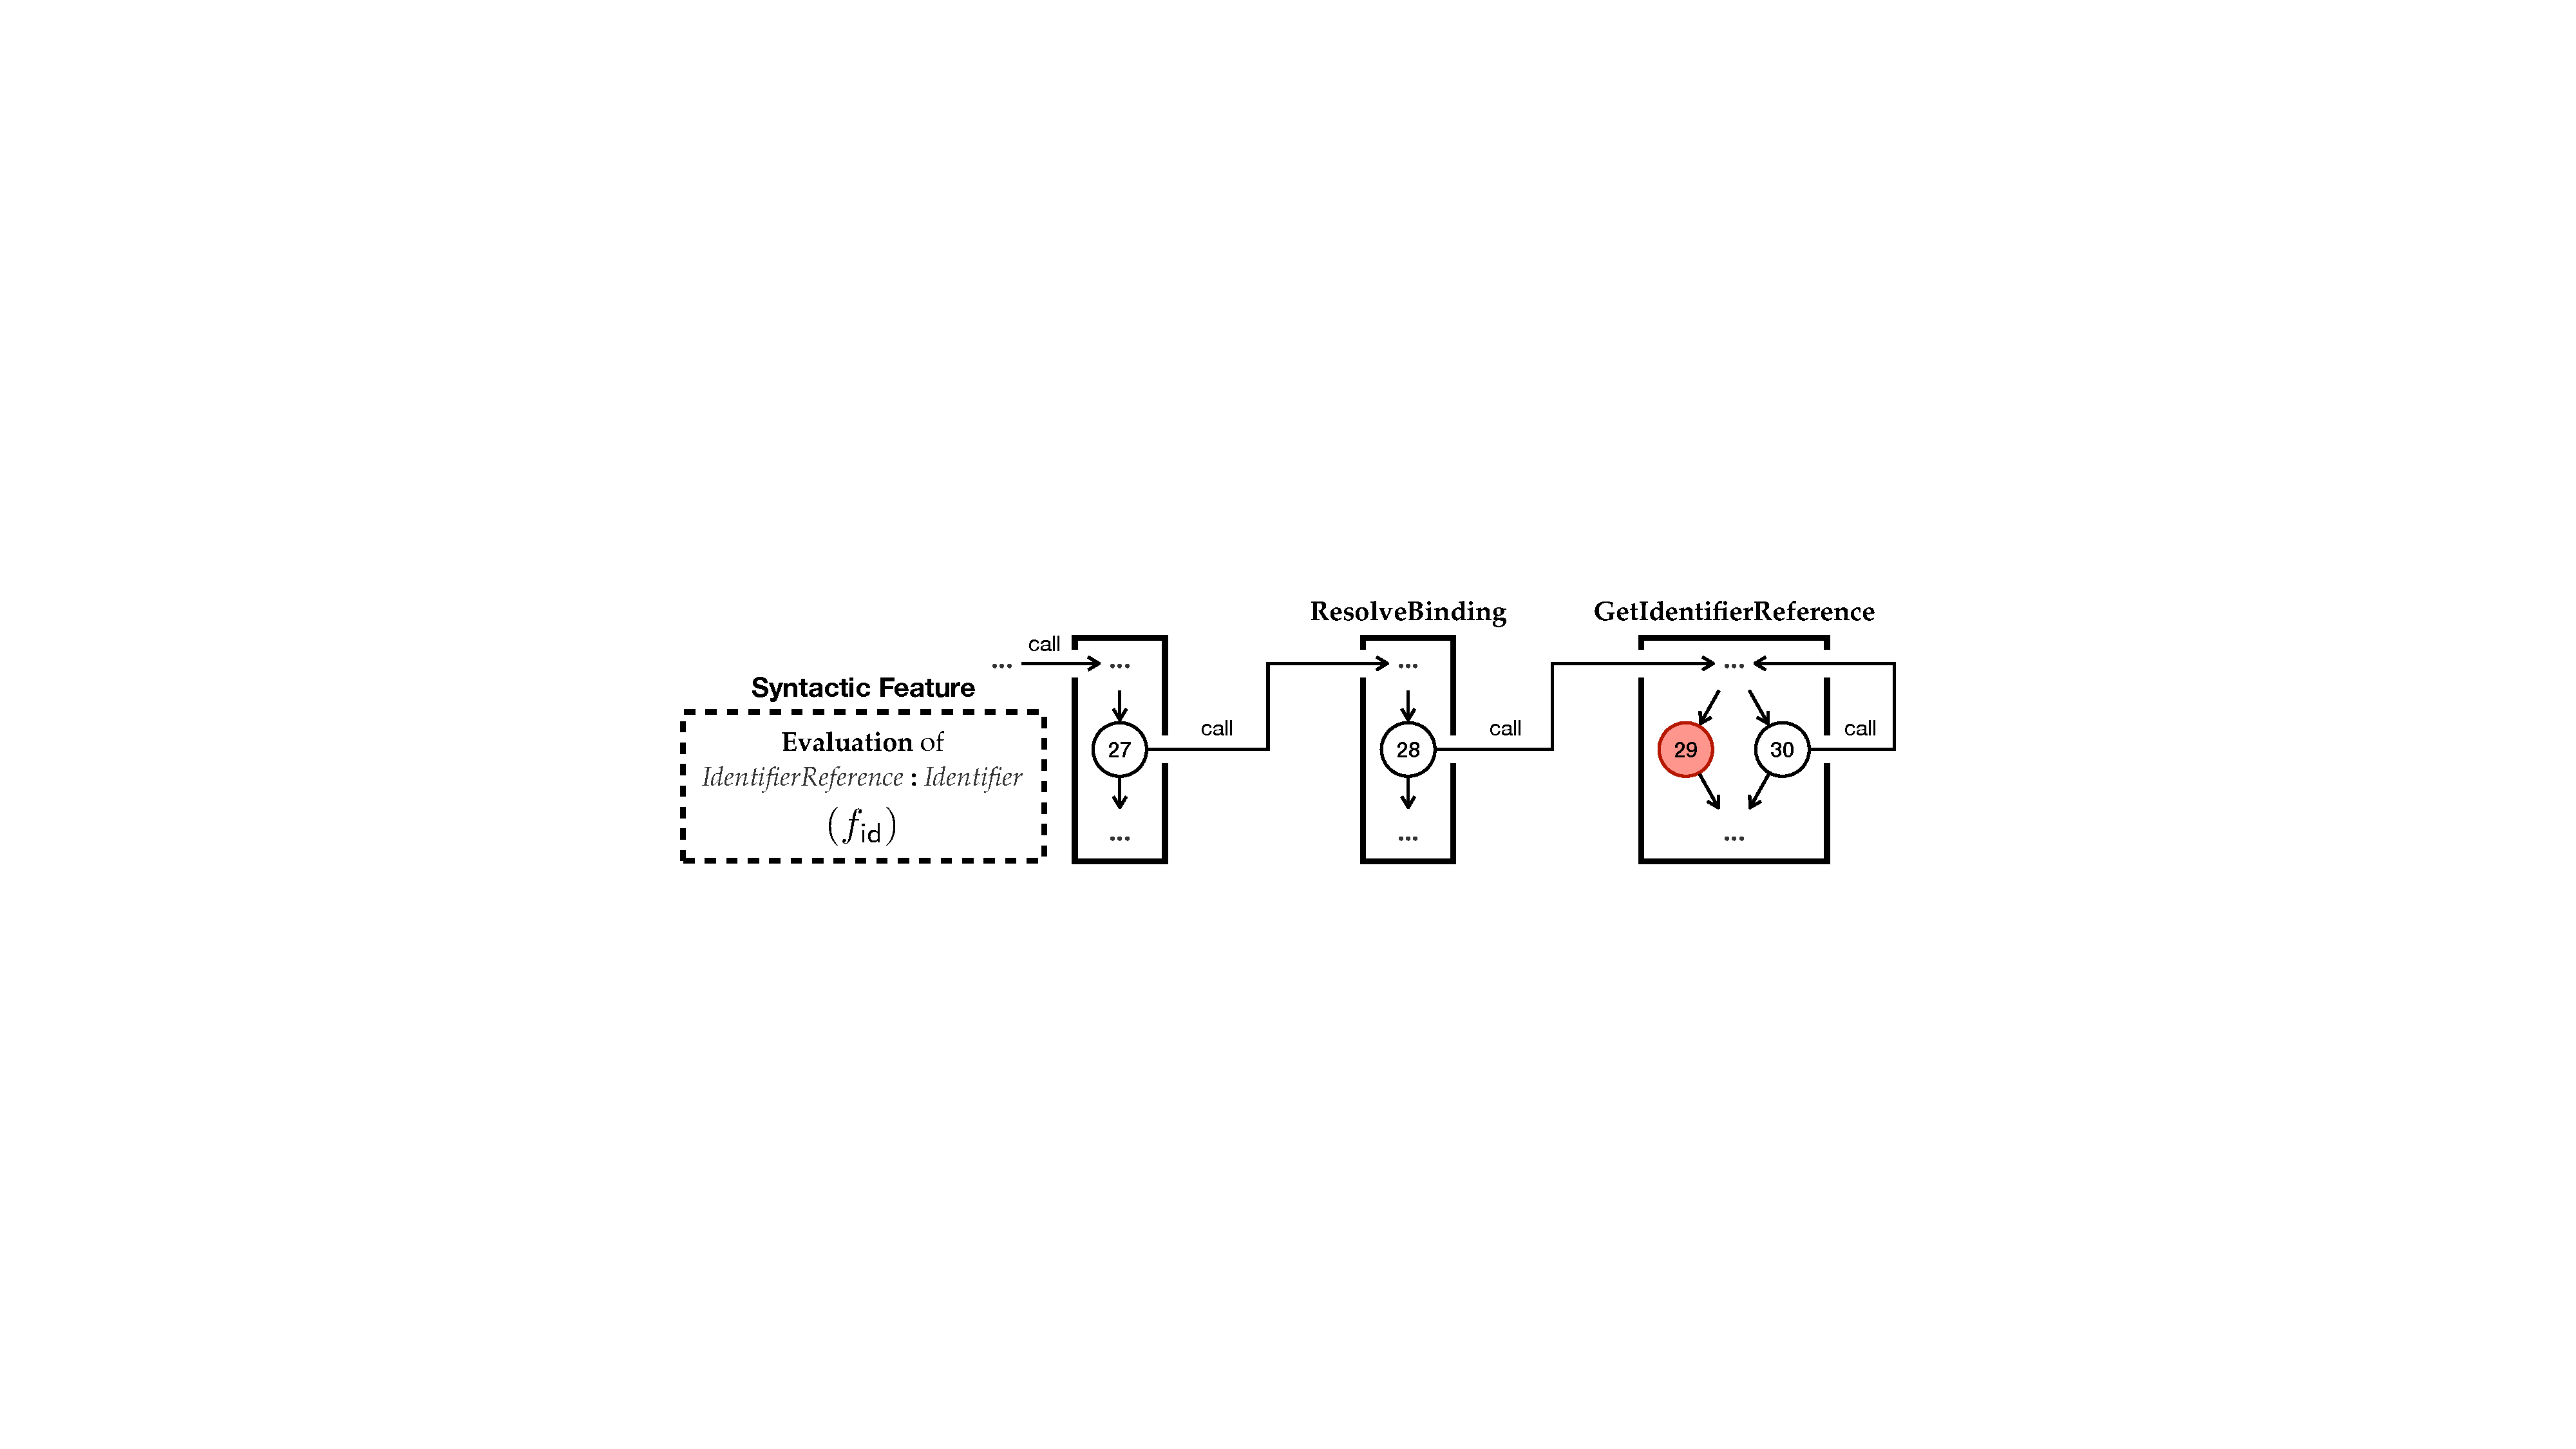
\includegraphics[width=0.8\textwidth]{img/spec-cfg-id}
\vspace*{-.5em}
  \caption{
Excerpt from the CFG of abstract algorithms for \esnt{IdentifierReference}
  }
  \label{fig:spec-cfg-id}
\vspace*{-1em}
\end{figure}

We show two examples for FCPS node coverage criteria.
%
First, consider the following two JavaScript programs as tests with the CFG in
Figure~\ref{fig:spec-cfg}:
%
\begin{equation}\label{equ:fcps-example1}
    \test_0 = \jscode{2n + 1} \qquad \test_1 = \jscode{1 + 2n}
\end{equation}
%
If we use FS node coverage criterion $\fnodecov{\graph}$, both tests $\test_0$
and $\test_1$ cover the same FS-TR $(21, \addfeat)$, and one of them might be
removed in the program pool.
%
However, if we use FCPS node coverage criterion $\fcpnodecov{\graph}$, $\test_0$
and $\test_1$ cover different FCPS-TRs $(21, (\addfeat, [1, 8, 12]))$ and $(21,
(\addfeat, [1, 8, 14]))$, respectively.
%
The other example is about the cycles in the call-site stacks with the graph in
Figure~\ref{fig:spec-cfg-id}.
%
It depicts an excerpt from the CFG of abstract algorithms in ES13 transitively
used in $\idfeat$, a syntactic feature defined by the first alternative of
\esnt{IdentifierReference} and its \textbf{Evaluation} SDO. 
%
Assume that we do not remove cycles in the feature-call-paths $\fcpset$ during
the extraction algorithm $\extfcp$.
%
Then, since the algorithm \textbf{GetIdentifierReference} contains a
self-recursion, there exists an infinite number of possible feature-call-paths
from $\idfeat$ to the node labeled 29:
%
\begin{equation}\label{fcp-inf-example}
  (\idfeat, [27, 28]) \qquad
  (\idfeat, [27, 28, 30]) \qquad
  (\idfeat, [27, 28, 30, 30]) \qquad
  \cdots
\end{equation}
%
Thus, we remove cycles in feature-call-paths to resolve this issue, and there
exists only two possible feature-call-paths: $(\idfeat, [27, 28])$ and
$(\idfeat, [27, 28, 30])$.

%----------------------------------------%

Similar to the extension of FS coverage criteria to $k$-FS coverage criteria,
we define $k$-FCPS coverage criteria by extending $\extfcp$ into $\extfcps{k}:
\css{\patset{\graph}} \rightarrow \fcpset^{\leq k}$:
%
\begin{equation}\label{equ:extfcps}
  \extfcps{k}([\node_1, \cdots, \node_m]) = \left\{
    \begin{array}{ll}
      (\epsilon, \epsilon) & \tif k = 0 \vee m = 0\\

      (\feats \cdot \feat, [\node_m]) & \tif \featmap(\node_m) = \feat \wedge
      \extfcps{k-1}([\node_1, \cdots, \node_{m-1}]) = (\feats, \_)\\

      \fcps & \tif \fcps = (\epsilon, \epsilon)\\

      (\feats, [\node'_0, \cdots, \node'_i]) &
      \tif \fcp = (\feats, [\node'_0, \cdots, \node'_{m'}]) \wedge
      \exists i. \tst \node'_i = \node_m\\

      (\feats, \nodes \cdot \node_m) & \tif \fcp = (\feats, \nodes)\\
    \end{array}
  \right.
\end{equation}
%
where $\fcpset^{\leq k} = \featset^{\leq k} \times \css{\patset{\graph}}$ is a
set of extended feature-call-paths, and $\fcps = \extfcps{k}([\node_1, \cdots,
\node_{m-1}])$.

%----------------------------------------%

\begin{definition}[$k$-Limiting Feature-Call-Path-Sensitive ($k$-FCPS)
  Coverage Criteria]\label{def:k-fcps-cov}
  For a given $\cov{\graph} = (\trset{\graph}, \cover)$, the
  \textit{$k$-limiting feature-call-path-sensitive ($k$-FCPS) coverage}
  criterion $\kfcpcov{k}{\graph} = (\kfcptrset{k}{\graph}, \cover)$ is defined
  as follows:
  \begin{itemize}
    \item the set of \textbf{$k$-feature-call-path-sensitive test requirements
      ($k$-FCPS-TRs)} $\kfcptrset{k}{\graph}$ is a set of original TRs tagged
      with the extended feature-call-paths bounded by $k$:
$
        \kfcptrset{k}{\graph} = \trset{\graph} \times \fcpset^{\leq k}
$
    \item a path $\pat$ \textbf{covers} a $k$-FCPS-TR $(\tr, \fcps)$ when $\pat$
      covers the original TR $\tr$ and $\fcps$ is the extended feature-call-path
extracted from $\pat$ bounded by $k$:
\[
        \pat \cover (\tr, \fcps) \iff \pat \cover \tr \wedge
        \extfcps{k}(\css{\pat}) = \fcps
\]
  \end{itemize}
\end{definition}

%----------------------------------------%

\begin{figure}
  \centering
\scriptsize
  \begin{tikzpicture}[every node/.style={draw=none}]
    \node (base)   at (0,1) {$\cov{\graph}=\kfcov{0}{\graph}=\kfcpcov{0}{\graph}$};
    \node (1-fs)   at (3,0) {$\fcov{\graph}=\kfcov{1}{\graph}$};
    \node (2-fs)   at (6,0) {$\kfcov{2}{\graph}$};
    \node (k-fs)   at (8,0) {$\cdots$};
    \node (1-fcps) at (3,2) {$\fcpcov{\graph}=\kfcpcov{1}{\graph}$};
    \node (2-fcps) at (6,2) {$\kfcpcov{2}{\graph}$};
    \node (k-fcps) at (8,2) {$\cdots$};
    \path[->]
    (1-fs) edge node[auto] {(A)} (base)
    (2-fs) edge node[auto] {(A)} (1-fs)
    (k-fs) edge node[auto] {(A)} (2-fs)
    (1-fcps) edge node[auto] {(B)} (base)
    (1-fcps) edge node[auto] {(C)} (1-fs)
    (2-fcps) edge node[auto] {(B)} (1-fcps)
    (2-fcps) edge node[auto] {(C)} (2-fs)
    (k-fcps) edge node[auto] {(B)} (2-fcps);
  \end{tikzpicture}
\vspace*{-1em}
  \caption{
    Subsumption relations between $k$-FS and $k$-FCPS coverage criteria
  }
\vspace*{-1em}
  \label{fig:subs}
\end{figure}

We prove Theorem~\ref{thm:subs} for the subsumption relations
between $k$-FS and $k$-FCPS coverage criteria.
Figure~\ref{fig:subs} illustrates the relations using edges
annotated with equations in Theorem~\ref{thm:subs}.

%----------------------------------------%

\begin{lemma}\label{lem:subs}
  Consider two graph coverage criteria $\cov{\graph} = (\trset{\graph}, \cover)$
  and $\cov{\graph}' = (\trset{\graph}', \cover')$.
  %
  If there exists a valid TR $\tr \in \trset{\graph}$ that satisfies the following
  condition for each valid TR $\tr' \in \trset{\graph}'$:
  %
  \begin{equation}\label{equ:subs-lemma}
    \forall \test \in \testset. \; \test \cover \tr \Rightarrow \test \cover' \tr'.
  \end{equation}
  %
  Then, $\cov{\graph}$ subsumes $\cov{\graph}'$ ($\cov{\graph}
  \subs\cov{\graph}'$).
\end{lemma}
\begin{proof}
  Assume $T \sat \cov{\graph}$.
  %
  For a given valid TR $\tr' \in \trset{\graph}'$, let $\tr \in \trset{\graph}$
  be the valid TR satisfying (\ref{equ:subs-lemma}).
  %
  Then, there exists a test $\test \in T$ such that $\test \cover \tr$ because
  $\tr$ is valid and $T \sat \cov{\graph}$.
  %
  Finally, $\test \cover \tr'$.
\end{proof}

\begin{theorem}[Subsumption Relation]\label{thm:subs}
  For a given integer $k > 0$, the following three subsumption relations
  ($\subs$) between $k$-FS and $k$-FCPS coverage criteria satisfy:
  \[
    \text{(A)} \; \kfcov{k}{\graph} \subs \kfcov{(k-1)}{\graph} \qquad
    \text{(B)} \; \kfcpcov{k}{\graph} \subs \kfcpcov{(k-1)}{\graph} \qquad
    \text{(C)} \; \kfcpcov{k}{\graph} \subs \kfcov{k}{\graph}
  \]
\end{theorem}

\begin{proof}
  We prove (A) using Lemma~\ref{lem:subs}, and omit
  the other cases because their proofs are similar.
  %
  Let $k > 0$.
  %
  For a given valid $(k-1)$-FS-TR $(\tr, \feats)$, there exists a test $\test
  \in \testset$ such that $\test \cover (\tr, \feats)$ because $(\tr, \feats)$
  is valid.
  %
  There exists a prefix path $\pat$ of $\patmap{\graph}(\test)$ such that $\pat
  \cover (\tr, \feats)$ ($\because$ (\ref{equ:test-cover})).
  %
  Then, a $k$-FS-TR $(\tr, \extfeats{k}(\css{\pat}))$ satisfies the condition
  (\ref{equ:subs-lemma}) because of the inductive definition of $\extfeats{k}$
  in (\ref{equ:extfeats}).
  %
  Finally, $k$-FS coverage criteria subsume $(k-1)$-FS coverage criteria.
\end{proof}
